\section{Prototyping}

\paragraph{A prototype is a useful design tool for testing concepts, clarifying requirements, and starting user interaction and feedback.
Prototyping methods can be categorized by fidelity—ranging from low-fidelity sketches to high-fidelity digital mockup.}

\subsection{Low-fidelity prototypes}

\paragraph{Low-fidelity prototypes, which often consist of simple sketches particularly valuable in the early stages of design}

\begin{figure}[h]
    \centering
    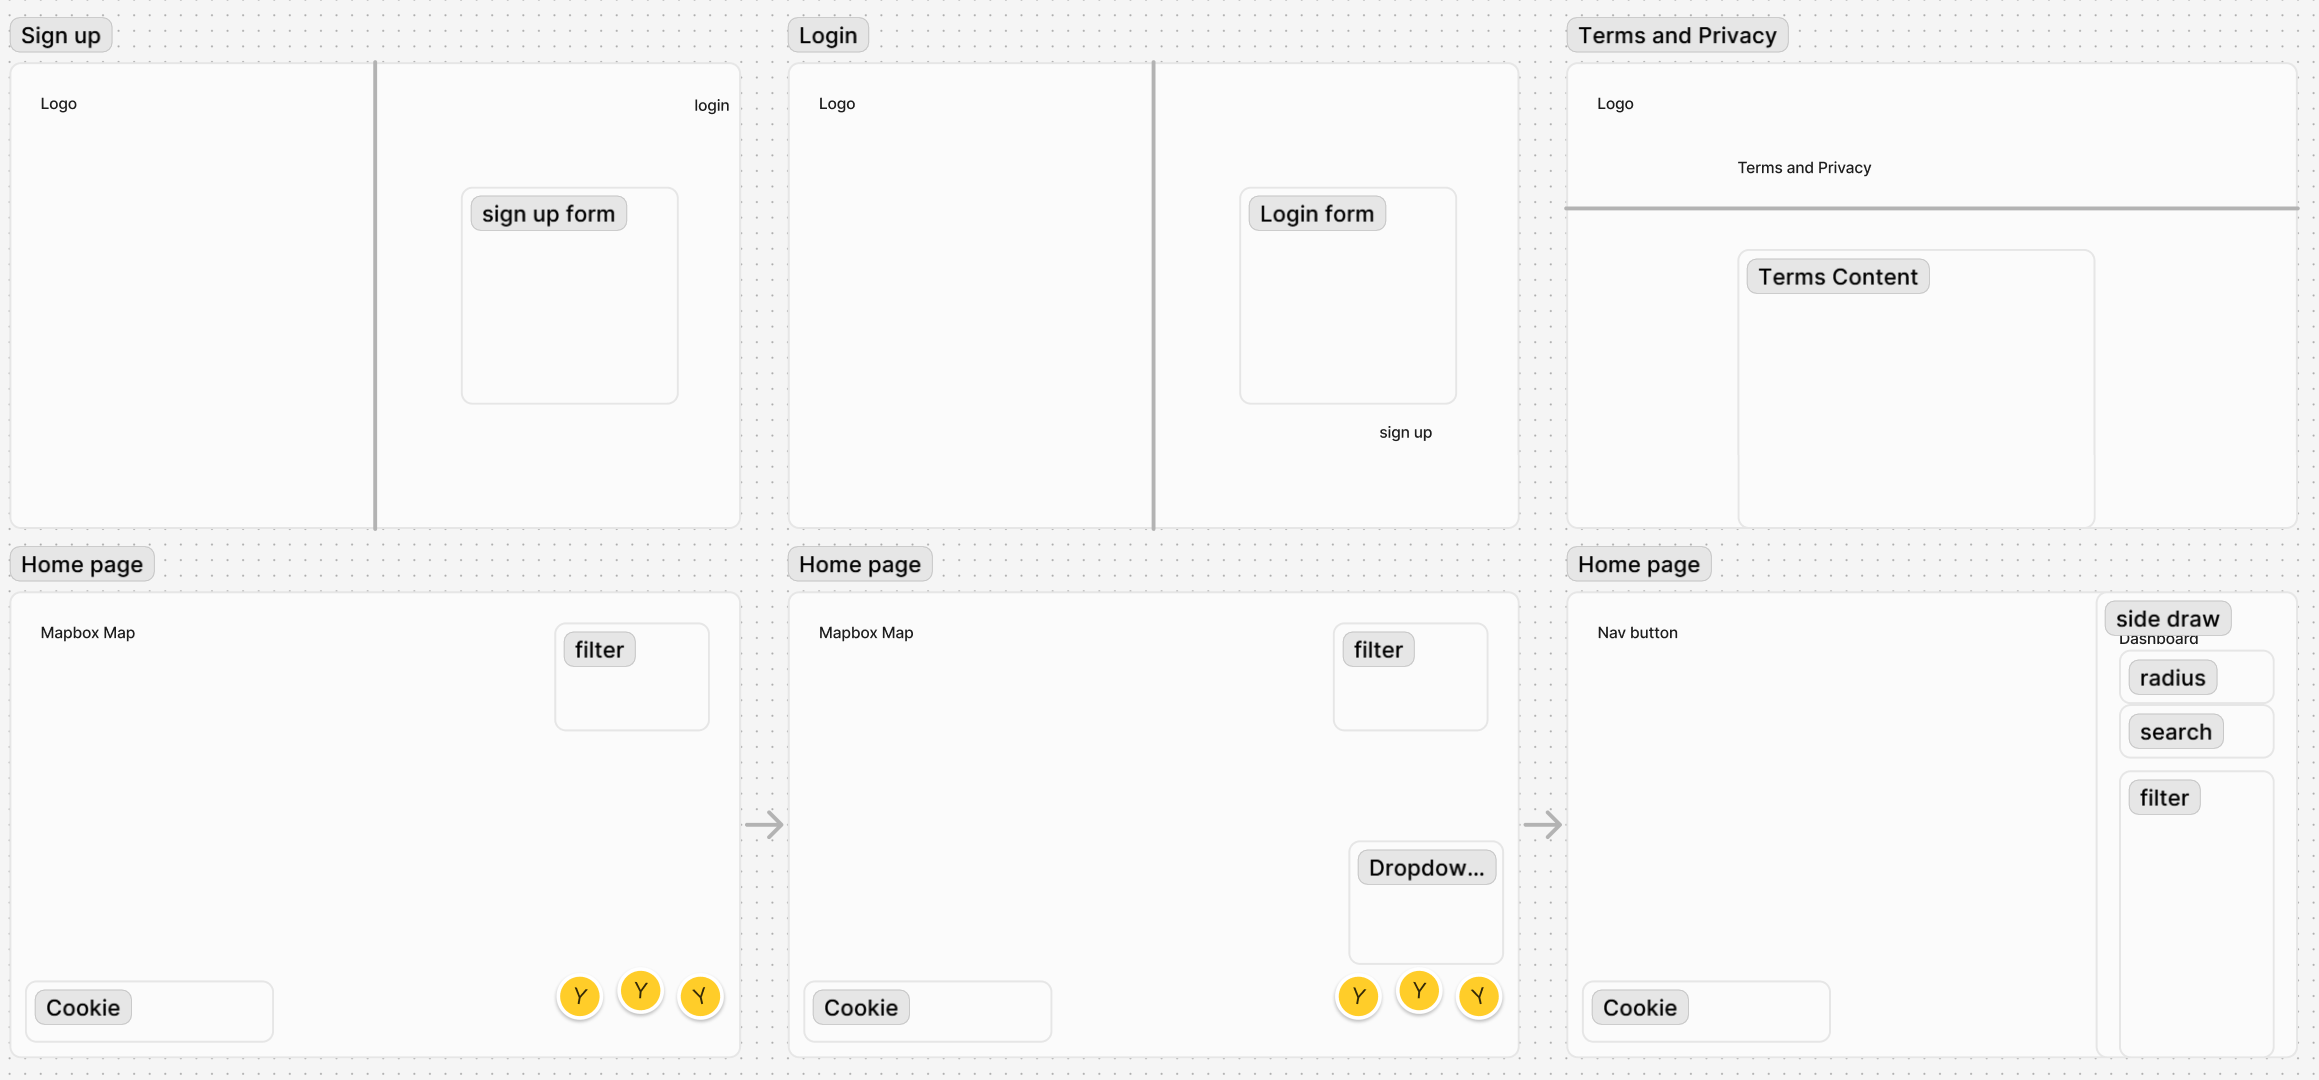
\includegraphics[width=\textwidth]{images/sketch.jpg}
    \caption{This is a sample caption for the image.}
    \label{fig:sample-image}
\end{figure}